\documentclass[letterpaper,12pt]{article}
\usepackage{array}
\usepackage{threeparttable}
\usepackage{fancyhdr,lastpage}
\pagestyle{fancy}
\lhead{}
\chead{}
\rhead{}
\lfoot{}
\cfoot{}
\rfoot{\footnotesize\textsl{Page \thepage\ of \pageref{LastPage}}}
\renewcommand\headrulewidth{0pt}
\renewcommand\footrulewidth{0pt}
\usepackage[format=hang,font=normalsize,labelfont=bf]{caption}
\usepackage{listings}
\lstset{frame=single,
  language=Python,
  showstringspaces=false,
  columns=flexible,
  basicstyle={\small\ttfamily},
  numbers=none,
  breaklines=true,
  breakatwhitespace=true
  tabsize=3
}

\usepackage{geometry}
\geometry{letterpaper,tmargin=1in,bmargin=1in,lmargin=1in,rmargin=1in}
%\renewcommand\headrulewidth{2pt}
%\renewcommand\footrulewidth{2pt}
\usepackage{amsmath}
\usepackage{amssymb}
\usepackage{amsthm}
\usepackage{mathtools}
\usepackage{pdflscape}
\usepackage{harvard}
\usepackage{setspace}
\usepackage{float,color}
%\usepackage{enumitem}
\usepackage[pdftex]{graphicx}
\usepackage{hyperref}
\hypersetup{colorlinks,linkcolor=red,urlcolor=blue}
\theoremstyle{definition}
\newtheorem{theorem}{Theorem}
\newtheorem{acknowledgement}[theorem]{Acknowledgement}
\newtheorem{algorithm}[theorem]{Algorithm}
\newtheorem{axiom}[theorem]{Axiom}
\newtheorem{case}[theorem]{Case}
\newtheorem{claim}[theorem]{Claim}
\newtheorem{conclusion}[theorem]{Conclusion}
\newtheorem{condition}[theorem]{Condition}
\newtheorem{conjecture}[theorem]{Conjecture}
\newtheorem{corollary}[theorem]{Corollary}
\newtheorem{criterion}[theorem]{Criterion}
\newtheorem{definition}[theorem]{Definition}
\newtheorem{derivation}{Derivation} % Number derivations on their own
\newtheorem{example}[theorem]{Example}
\newtheorem{exercise}[theorem]{Exercise}
\newtheorem{lemma}[theorem]{Lemma}
\newtheorem{notation}[theorem]{Notation}
\newtheorem{problem}[theorem]{Problem}
\newtheorem{proposition}{Proposition} % Number propositions on their own
\newtheorem{remark}[theorem]{Remark}
\newtheorem{solution}[theorem]{Solution}
\newtheorem{summary}[theorem]{Summary}
\numberwithin{equation}{section}
\bibliographystyle{aer}
\newcommand\ve{\varepsilon}
\newcommand\boldline{\arrayrulewidth{1pt}\hline}
\newcommand{\q}[1]{``#1''}

\def\changemargin#1#2{\list{}{\rightmargin#2\leftmargin#1}\item[]}
\let\endchangemargin=\endlist 

\usepackage{graphicx}
\graphicspath{ {images/} }

\usepackage{enumerate}
%\usepackage[shortlabels]{enumerate}
\setlength{\parindent}{24pt}
%\renewcommand{\baselinestretch}{2.0}
\usepackage{lipsum} % just for the example
\makeatletter
\newcommand{\verbatimfont}[1]{\renewcommand{\verbatim@font}{\ttfamily#1}}
\makeatother
%\usepackage{enumitem}
\usepackage{float}

\verbatimfont{\small}%


\begin{document}

\begin{flushleft}
   \textbf{\Large{Problem Set \#3}} \\
   MACSS 30100 \\
   Luxi Han, 10449918\\
\end{flushleft}

\textbf{[Note]: The \(\mu\) and \(\sigma\) in the legend plotted here is the expectation and standard deviation of the log normal pdf. It is NOT the mean and standard deviation of the income distribution!!}\, \, \\
\, \\

\noindent \textbf{\large Problem 1}\par

\begin{enumerate} [\bfseries (a)]
\item The following graph is the histogram for the income of the MACSS cohort:\\
	\begin{figure}[H]
    		\centering
		\fbox{\resizebox{4.75in}{3in}{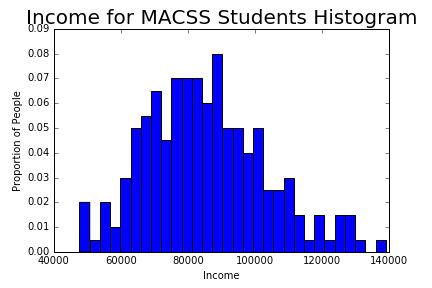
\includegraphics{hist_income}}}\
    		\caption{Histogram of Income of MACSS Students}
	\end{figure}\par
	
\item The GMM estimator of two moment conditions: the log normal parameters are: \(\mu = 11.332, \, \sigma = 0.209\). \\
The data moment is: \(\mu_{data} = 85276.824, \, \sigma_{m odel} = 323731572.230\).\\
The model moment is \(\mu_{model} = 85276.819, \, \sigma_{model} = 23731572.235\)\\
The value of the criterion function is \(1.47304603e-09\)\par
	\begin{figure}[H]
    		\centering
		\fbox{\resizebox{5in}{3in}{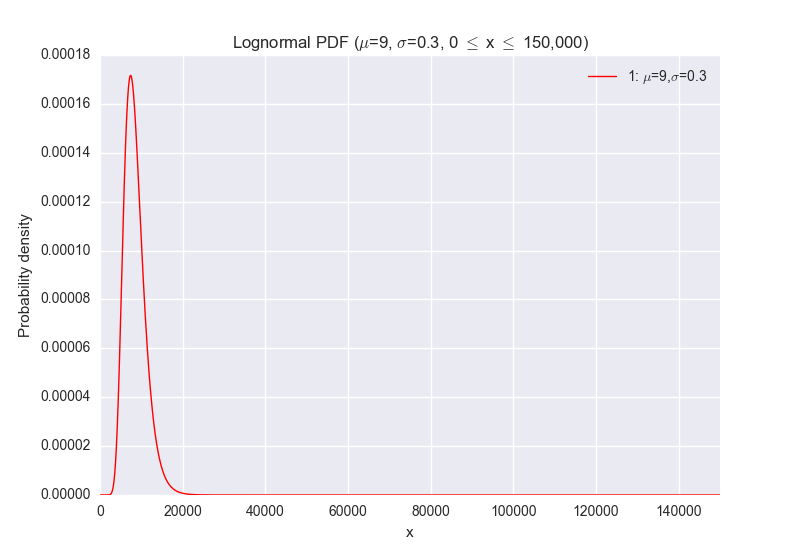
\includegraphics{1b}}}\
    		\caption{Income PDF of Two Moment Conditions}
	\end{figure}\par

\item The GMM estimator of two moment conditions using TWO-STEP variance covariance matrix is: the log normal parameters are: \(\mu = 11.331, \, \sigma = 0.209\). \\
The model moment is \(\mu_{model} = 85277.076, \, \sigma_{model} = 323732317.170\)\\
The value of the criterion function is \(0.00192164\)\par
The plotted graph is as following:\\
	\begin{figure}[H]
    		\centering
		\fbox{\resizebox{5in}{3in}{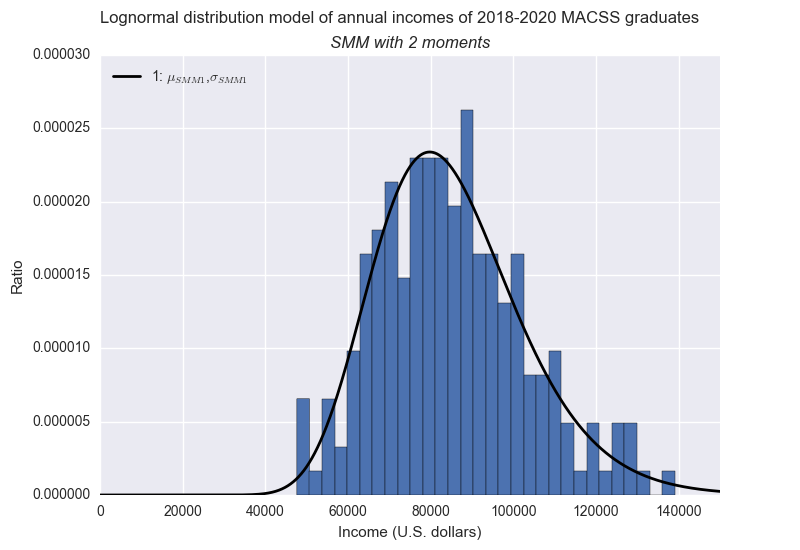
\includegraphics{1c}}}\
    		\caption{Income PDF of Two Moment Conditions(TWO-STEP)}
	\end{figure}\par

\item  The data and model moments are reported as below:\\
Data moment:\\
The proportion of students whose income is below \$75000 is: 0.3 \\
The proportion of students whose income is between \$75000 and \$100000 is: 0.5\\
The proportion of students whose income is above \$100000 is: 0.2\\
\\
Model Moment:\\
The proportion of students whose income is below \$75000 is: 0.30000001   \\
The proportion of students whose income is between \$75000 and \$100000 is: 0.5000001   \\
The proportion of students whose income is above \$100000 is: 0.19999989 \par
The value of the criterion function is 3.71437920e-13\\
The following is the PDF graph:\\
	\begin{figure}[H]
    		\centering
		\fbox{\resizebox{5in}{3in}{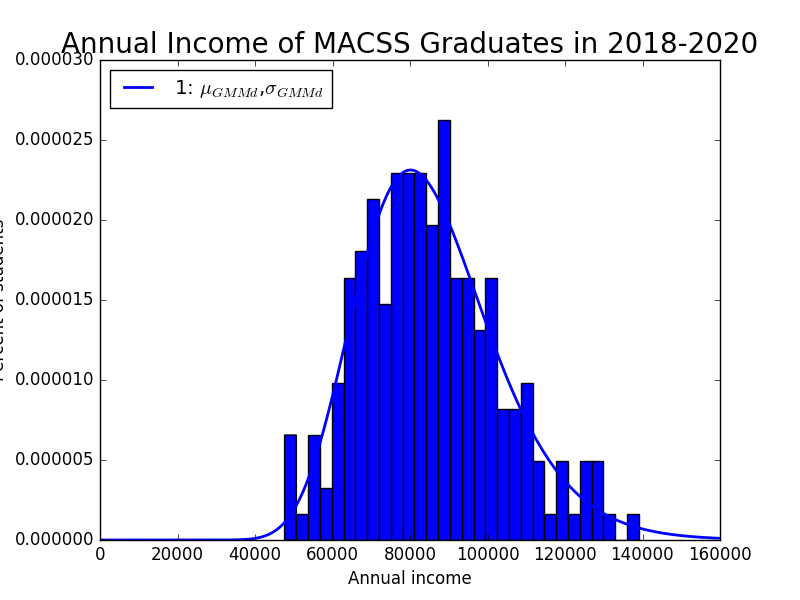
\includegraphics{1d}}}\
    		\caption{Income PDF of Three Moment Conditions}
	\end{figure}\par

\item We have the following result:\\
The model moments using the variance covariance weighting matrix is as following:\\
Model Moment:\\
The proportion of students whose income is below \$75000 is: 0.30040381   \\
The proportion of students whose income is between \$75000 and \$100000 is:  0.49963281    \\
The proportion of students whose income is above \$100000 is: 0.19996338  \par
The value of the criterion function is 2.38464060e-06\\
The following is the PDF graph:\\
	\begin{figure}[H]
    		\centering
		\fbox{\resizebox{5in}{3in}{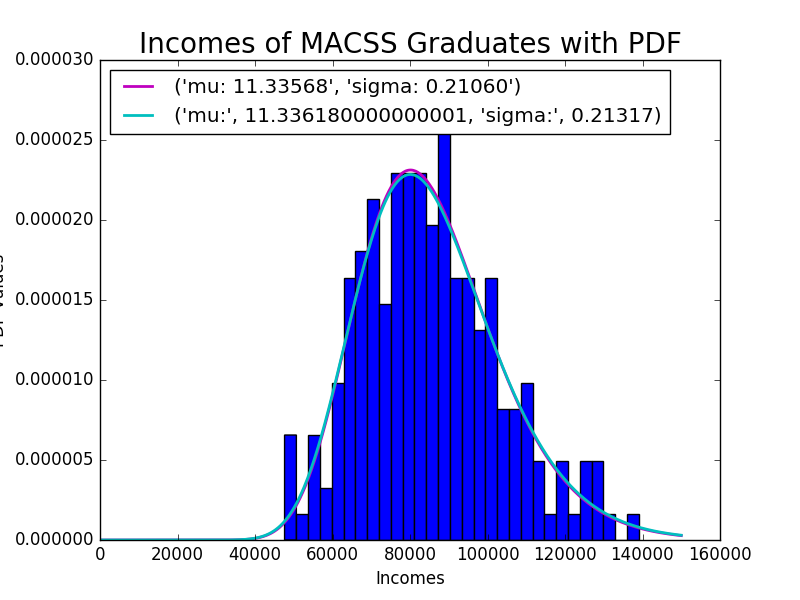
\includegraphics{1e}}}\
    		\caption{Income PDF of Three Moment Conditions(TWO-STEP)}
	\end{figure}\par
\item
As I tried to compute the GMM estimator, the minimizer didn't perform well. Using different methods lead to different result. The method I used is Nelder-Mead. It generates the above results. But again, this may not be the minimized version since the criterion function may be very lumpy.\par
According to the criterion value function, the result computed in part d) is the one with the best performance. The two TWO-STEP estimators all underperform the original ones. This is unexpected. This may be as the result that the original method is already close to the model moments. This may affect the usefulness of the weighting matrix. All in all, the original GMM estimator using the three moment condition is the best.\par
\end{enumerate}

\noindent \textbf{\large Problem 2}\par
The estimators are:\\
\begin{align*}
\beta_0 &= 0.252\\
\beta_1 &= 0.013\\
\beta_2 &= 0.401\\
\beta_3 &= -0.010\\
\end{align*}
The value of the criterion function is \(0.0018\).


\end{document}